%File: technical_supplement.tex
\documentclass[letterpaper]{article}
\usepackage[submission]{aaai2027}
\usepackage[hyphens]{url}
\usepackage{booktabs}
\usepackage{graphicx}
\graphicspath{{figures/}}
\usepackage{amsmath}
\usepackage{amssymb}
\usepackage{xspace}
\usepackage{natbib}
\urlstyle{rm}
\def\UrlFont{\rm}
\frenchspacing
\pdfinfo{/TemplateVersion (2027.1)}
\setcounter{secnumdepth}{2}
\newcommand{\Bench}{\textsc{SelectGround-Bench}\xspace}
\newcommand{\Method}{\textsc{ReGate}\xspace}
\title{Technical Supplement for ReGate: Mitigating Hallucinations in Visual Grounding via Metamorphic Counterfactual Supervision}
\author{Anonymous Submission}
\affiliations{}
\begin{document}
\maketitle

This supplement provides the complete implementation, construction, prompt, protocol, and extended-analysis details supporting the main paper.
\appendix

\section{Structured Output and Parsing Protocol}
\label{sec:structured_output}
The three semantic outcomes use one fixed machine-readable schema. Supported queries return
{\ttfamily\small\sloppy\noindent
\{"decision":"answer", "label":"...", "box":[x1,y1,x2,y2]\}
\par}
and unsupported queries return
{\ttfamily\small\sloppy\noindent
\{"decision":"abstain", "reason":"wrong\_object|no\_target"\}
\par}
Here the vertical bar denotes a choice between the two legal values rather than a literal output. The symbolic value \texttt{wrong\_object} serializes visual contradiction and \texttt{no\_target} serializes target unavailability. Boxes use relative coordinates in $[0,1000]^4$. Before label comparison, predicted and reference labels are normalized symmetrically by lowercasing, replacing underscores with spaces, removing punctuation and the generic modifiers \texttt{leaf}, \texttt{plant}, and \texttt{disease}, and collapsing whitespace.

Each of the five task-specific autoregressive interfaces uses the same parser and receives at most one identical format-only retry after invalid JSON or an illegal box; the retry preserves the semantic instruction and is included in parse success and inference cost. GPT-5.6 uses the same parser on one accepted response per record, with transport retries only and no format retry or voting. \Method's discriminative gate always supplies a valid selective state and requires no retry; its supported route invokes the adapted generator under the base structured instruction. Metric treatment of routed candidates is specified in Section~\ref{sec:metric_operating_details}.

\section{Training, Checkpoint, and Gate Protocol}
\label{sec:two_stage_protocol}
For each image--query input, the readout is the hidden state at the last non-padding token of the generation prompt, immediately before the first assistant-response token. During teacher-forced training this is the token immediately preceding the first non-masked response label; during inference it is the final valid token produced by the chat template with the generation prompt appended. The training-stage gate uses \texttt{hidden\_states[27]}, where index zero is the embedding output and API index 27 is the output of transformer block 26 under zero-based block numbering.

During joint adaptation, normalization statistics are computed from a deterministic 2,000-record subset of frozen-backbone training representations. LoRA uses $r=16$, $\alpha=32$, dropout $0.05$, learning rate $10^{-4}$, and up to six epochs. The joint objective combines teacher-forced structured-output loss with the auxiliary weighted three-state loss, whose coefficient increases linearly from zero to $0.4$ during the first ten optimizer steps; state weights are $[1.0,1.5,1.0]$.

Stage~1's auxiliary head and Stage~2's final inference gate use the same $4096\!\rightarrow\!512\!\rightarrow\!256\!\rightarrow\!3$ MLP architecture with GELU activations and dropout $0.1$ after each hidden layer, but are fitted at their respective stages; only the Stage~2 gate supplies reported \Method decisions. Including biases, this architecture has $2{,}229{,}763$ trainable parameters (2.23M, or $0.028\%$ of the backbone). The Stage~1 objective is optimized sample-wise: controlled records and their state labels encode the metamorphic counterfactual structure. Because same-source groups assign different evidence states under shared provenance, source identity alone is insufficient to satisfy all group labels; the supervision therefore promotes query--evidence compatibility.

Before Stage~1, a capacity-controlled coarse probe is restricted to the training-side diagnostic pool: identical logistic classifiers are fitted on source-group-disjoint probe-fitting records, and three evenly spaced candidate depths (API indices 9, 18, and 27) are compared on probe-development records. The 296-record reserved holdout, formal benchmark development/test records, and external probes are excluded; index 27 performs best and is fixed for joint adaptation. The fixed first 100 records of the formal $2{,}408$-record benchmark development pool then evaluate the six epoch checkpoints by teacher-forced language-model loss, selecting the Grouped and Independent minimum-loss checkpoints (training-step identifiers 444 and 222, respectively).

After checkpoint retention, the adapted backbone and grounding generator are frozen. The post-adaptation depth diagnostic is built from 372 source-image groups containing supported anchors and visual-contradiction records. It keeps all 973 contradiction records, up to two supported anchors per group, and up to one target-unavailable control, yielding 2,032 records (973 contradiction, 688 supported, and 371 unavailable). Fifty-five groups (296 records) are reserved as an untouched holdout and enter neither probe fitting nor depth selection; no number reported in this paper is computed on them. The remaining 317 groups (1,736 records) are split by source group into 292 groups (1,599 records) for probe fitting and 25 groups (137 records) for probe development; the group-disjoint split therefore yields 1,599 fitting records. Logistic probes with $C\in\{0.01,0.1,1.0\}$ scan all 36 depths. The worst-state criterion selects API index 27 globally, with $m_{27}=0.9574$; representative depths appear in Table~\ref{tab:depth_scan}. These training-side diagnostic partitions are distinct from the formal benchmark development and test splits; the probes are used only to confirm the readout position and are absent from inference.

\begin{table}[t]
\centering
\small
\setlength{\tabcolsep}{1.6mm}
\begin{tabular}{crcrcrcr}
\toprule
API & $m_\ell$ & API & $m_\ell$ & API & $m_\ell$ & API & $m_\ell$ \\
\midrule
1 & .638 & 14 & .785 & 18 & .923 & 22 & .936 \\
26 & .936 & \textbf{27} & \textbf{.9574} & 28 & .936 & 36 & .915 \\
\bottomrule
\end{tabular}
\caption{Representative post-adaptation depth diagnostic; API index 27 is the global maximum.}
\label{tab:depth_scan}
\end{table}

Final normalization statistics are recomputed from all $7{,}072$ adapted training representations, and the $4096\!\rightarrow\!512\!\rightarrow\!256\!\rightarrow\!3$ gate is refitted with cross-entropy. Gate early stopping uses a seed-42 class-stratified 100-record sample (34/33/33 by state) from the same formal $2{,}408$-record benchmark development pool. Both model-selection samples are drawn exclusively from formal benchmark development records. After model fitting, the development-selected operating threshold is chosen on all $2{,}408$ formal benchmark development records. No test or external-probe record enters checkpoint, gate, or threshold selection.

\section{Metric and Operating-Point Details}
\label{sec:metric_operating_details}

Let $\mathcal D_{\mathrm{sup}}$ and $\mathcal D_{\mathrm{unsup}}$ be the fixed supported and unsupported reference universes. In addition to the main-paper metrics, the construction analysis uses A\_FU (the supported-query non-answer rate on $\mathcal D_{\mathrm{sup}}$), U\_Abs (the valid-abstention rate on $\mathcal D_{\mathrm{unsup}}$), AAC (the mean $C_G$ on $\mathcal D_{\mathrm{sup}}$), and U\_Reason (the mean reason-correctness indicator $C_R$ on $\mathcal D_{\mathrm{unsup}}$). For box-free supported records, AAC uses semantic correctness $C_S$ in place of $C_G$. Selective MCC is the standard Matthews coefficient of the binary answer/non-answer confusion matrix, with value zero when its denominator vanishes.

For generative interfaces, a final invalid output is a non-answer selection for FCA, retention, A\_FU, and MCC; it is not a valid abstention and receives no semantic, reason, or grounding credit. Hence FCA and U\_Abs need not sum to one. For \Method, the gate defines all binary selection metrics: a final abstention-form or malformed candidate on an answer route remains an answer selection, but receives zero semantic, reason, and grounding credit.
Base and SFT native are format-valid on all comprehensive records.

For \Method, the reported fixed operating point uses three-class argmax, while thresholded routing answers when $p_A\geq\tau$ and otherwise selects $\arg\max_{s\in\{C,U\}}p_s$. The threshold $\tau=0.9888$ is selected on all $2{,}408$ formal benchmark development records at the SFT-native development retention of $86.05\%$ and then frozen. On the comprehensive test, it attains $88.96\%$ retention and $4.54\%$ FCA, versus SFT native's $85.11\%$ and $9.45\%$, a $52.0\%$ relative FCA reduction with higher supported coverage.

Complete test-set sweeps provide operating-characteristic diagnostics. At the empirical point matching SFT-native test retention, comprehensive FCA is $0.036$ versus $0.094$ (a $61.6\%$ reduction) and Strict-3 is $0.866$. The corresponding matched FCA values are $0.197/0.155$ for ReGate/SFT native on PlantWild and $0.050/0.044$ on RefCOCOg. Figure~\ref{fig:full_operating_curves} reports all three curves; these curve-matched values characterize routing behavior, whereas the development-selected threshold above is the held-out operating result.

\begin{figure*}[t]
\centering
\begin{minipage}[t]{0.32\textwidth}
\centering
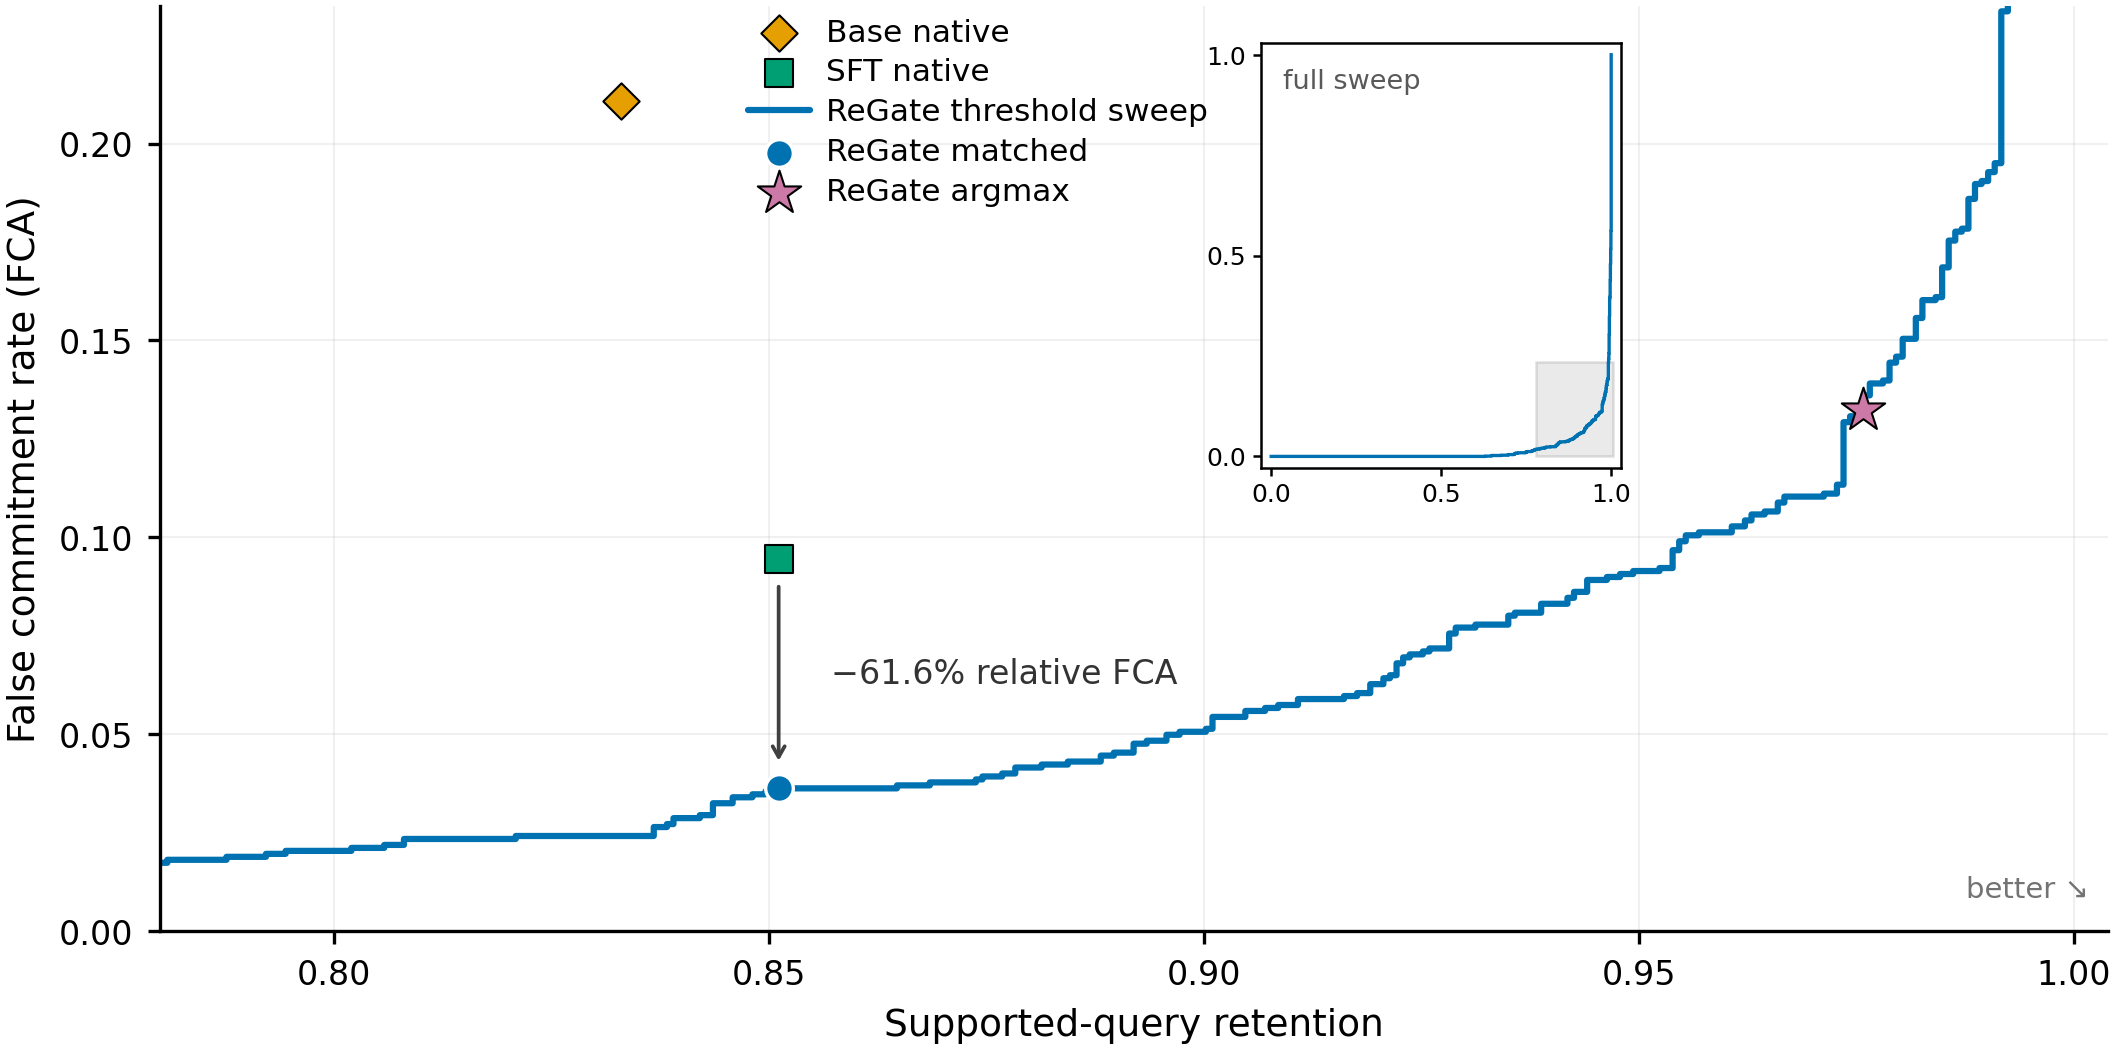
\includegraphics[width=\linewidth]{fig_hallucination_retention.png}\par
\centering\textbf{(a) Comprehensive}
\end{minipage}\hfill
\begin{minipage}[t]{0.32\textwidth}
\centering
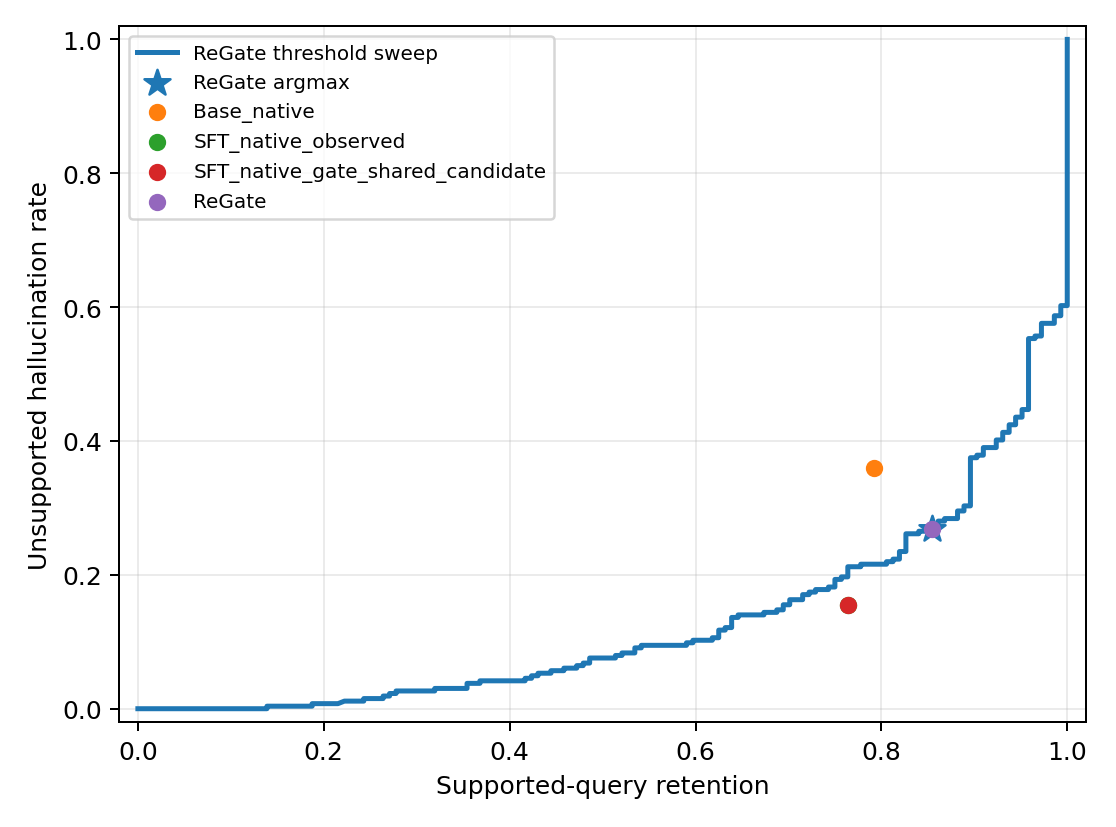
\includegraphics[width=\linewidth]{fig_hallucination_retention_plantwild.png}\par
\centering\textbf{(b) PlantWild}
\end{minipage}\hfill
\begin{minipage}[t]{0.32\textwidth}
\centering
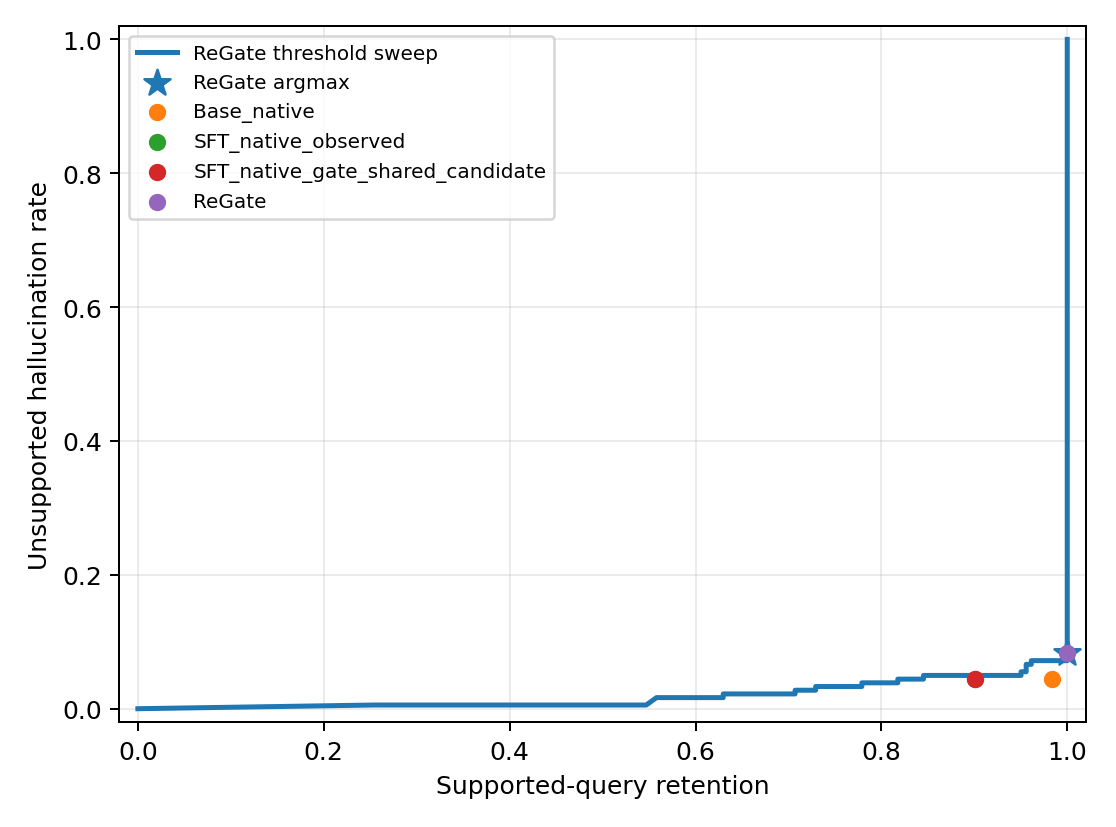
\includegraphics[width=\linewidth]{fig_hallucination_retention_refcocog.png}\par
\centering\textbf{(c) RefCOCOg}
\end{minipage}
\caption{Complete FCA--retention operating curves on Comprehensive, PlantWild, and RefCOCOg.}
\label{fig:full_operating_curves}
\end{figure*}

Strict-3 evaluates three-state semantic correctness and does not include localization. Relation-level MTS adds the applicable spatial requirement: T1--T3 require a supported decision, correct label, and IoU $\geq0.5$ in derived-image coordinates; \texttt{T4\_control} uses the same supported criterion; \texttt{T2\_occluded}, \texttt{T3\_occluded}, and \texttt{base\_occluded} require target unavailability; T5 and T6 require their designated abstention reasons; and supported T7 variants additionally require the spatial criterion. MTS is relation-stratified strict satisfaction against the construction-defined reference outcome, rather than prediction-to-prediction consistency, and therefore does not credit mutually consistent but jointly incorrect predictions. \texttt{T7\_ladder} aggregates its hard-labeled records, while group-level monotonicity is reported separately by L3.

\section{Data Construction and Label-Space Audit}
\label{sec:implemented_construction}

This section records the operators and routing rules implemented by the provided
PlantDoc and COCO builders. Hard-label geometric boxes use the normalized
$[0,1000]^4$ coordinate system after the relevant crop or transformation.
Answerable T4 dose records retain the source-image box in the top-level box
field and store the crop-remapped \texttt{crop\_target\_box} in metadata.

\subsection{Deterministic Relation Operators}

\paragraph{T1: paraphrasing.}
T1 changes only the query template; the image, target class, and GT box remain
fixed. The builder deterministically selects among ``Locate the \{label\} in
this image,'' ``Find the \{label\} and return its bounding box,'' and ``Where
is the \{label\} in the image?''

\paragraph{T2: photometric preservation.}
T2 applies brightness enhancement with factor $1.1$ followed by contrast
enhancement with factor $1.1$. The target class and GT box remain unchanged.
With the paired complete-crop-out option enabled
(\texttt{collinearity\_break=true}), a separate zero-visibility crop is also
generated from the transformed image as \texttt{T2\_occluded}.

\paragraph{T3: geometric equivariance.}
T3 applies a horizontal flip and mirrors the box as
\[
x'_1=1000-x_2,\quad x'_2=1000-x_1,\quad
y'_1=y_1,\quad y'_2=y_2.
\]
The paired complete-crop-out construction likewise generates
\texttt{T3\_occluded} by applying a zero-visibility crop with the mirrored box.

\paragraph{T4: target-evidence degradation and control.}
For PlantDoc, the builder first crops the target with approximately $10\%$
context and stores the remapped \texttt{crop\_target\_box} in metadata; mild
answerable dose records retain the source-image box in the top-level box field.
It then applies
Gaussian blur (radii $2,4,6,8$), pixelation (block sizes $4,6,10,12$), or
mean-color replacement to the target region. COCO uses Gaussian blur and
mean-color replacement on the target region in the full image. Every
target-degradation record is marked \texttt{dose\_only=true} and routed to the
separate dose-analysis pool (\texttt{dose\_pool.jsonl}), outside the hard-label
SFT and MTS sets.
\texttt{T4\_control} applies the same operator to a grid-selected background
region that avoids every annotated box, while retaining the original target,
label, and GT box as a supported hard-label record.

\paragraph{T5: cross-crop absent query.}
T5 keeps the image fixed and replaces the query with a class absent from its
annotations. For PlantDoc, the replacement must also have a different crop
prefix; four absent classes are selected deterministically per positive target.
The COCO builder selects two absent categories per positive target. T5 is
labeled \emph{target unavailable}.

\paragraph{T6: confusable same-crop query.}
T6 keeps the image unchanged and replaces only the queried class.
Alternatives come from configured same-crop disease sets for tomato, corn, and
apple. The builder reads all category annotations for the image and skips an
alternative if it is already annotated or lies outside the final retained label
space; this automatically excludes an already annotated alternative in
multi-disease images. T6 is labeled \emph{visual contradiction}; every admitted
record therefore satisfies the annotation-derived exclusion constraint
deterministically. A separate construction-consistency audit verifies the source
category, substituted query, and fixed same-crop mapping against these rules;
all T6 outcomes remain relative to the source annotations.

\paragraph{T7: crop-controlled visibility.}
T7 moves a crop boundary across the target box to request visible-area ratios
$1.0,0.75,0.5,0.25,$ and $0.0$. After integer-pixel cropping, the builder
recomputes the achieved visible ratio and remaps the retained GT box into crop
coordinates. \texttt{T7\_include} is a separate target-inclusion crop with
approximately $10\%$ context; \texttt{T7\_ladder} denotes the five requested
visibility levels.

\subsection{Hard-Label and Dose Routing}
\label{sec:visibility_routing}

The $1.0$ and $0.75$ T7 levels are supported hard-label records. At the nominal
$0.5$ level, achieved visibility determines routing: records with achieved
ratio at least $0.5$ enter the supported hard-label splits (PlantDoc: $483$;
COCO: $425$), while the remainder enter the dose pool (PlantDoc: $140$; COCO:
$142$). The $0.25$ level is dose-only. The $0.0$ crop fully excludes the target,
retains no box, and receives \emph{target unavailable} with
\texttt{reason=no\_target}.

These $483/425$ counts describe the complete PlantDoc/COCO build pools at the
nominal $0.5$ level before downstream training balancing. The final SFT assembly
samples 300 supported visibility-controlled records across the nominal $0.75$
and retained $0.5$ pools, as reported in the main paper's training-composition table.

Thus the T7 ladder's hard-labeled records comprise $1.0$, $0.75$, nominal $0.5$
with achieved visibility at least $0.5$, and $0.0$; the remaining nominal $0.5$
records and the $0.25$ level are dose-only. The separate L3 probe uses only the
$1.0$ and $0.0$ endpoints for fixed-point evaluation, yielding 331
endpoints (183 supported and 148 unavailable), while the remaining 419 records
at $0.75$, $0.5$, and $0.25$ are reserved for graded-response analysis. Integer-pixel feasibility
and record-level balancing leave 48 of 168 development groups and 55 of 183
test groups with all five levels. The dose analysis uses every available level
within each group and does not impute missing levels. This design separates
hard-label fixed-point evaluation from continuous response at intermediate
visibility levels.

\subsection{Explicit Same-Source Grouping Counts}
\label{sec:grouping_counts}

The explicitly grouped assembly contains $1{,}907$ training instances but
$1{,}671$ distinct serialized records. The difference is caused by 236
base-answer records reused by both the T6-anchor and T7 target-retaining
components.
\begin{table}[t]
\centering
\small
\begin{tabular}{lr}
\toprule
Component & Instances \\
\midrule
Original target-present anchors & 372 \\
Visual contradiction & 973 \\
Target-retaining visibility & 281 \\
Target-excluding visibility & 281 \\
\midrule
Grouped-instance total & 1,907 \\
Distinct serialized records & 1,671 \\
\bottomrule
\end{tabular}
\caption{Same-source grouping counts before contradiction resampling.}
\label{tab:explicit_grouping_counts}
\end{table}

The 973 unique contradictions comprise 594 tomato, 312 corn, and 67 apple
counterfactuals. Of 669 direct zero-visibility variants, 281 are explicitly
grouped and 388 provide additional target-exclusion supervision.

Before visual-contradiction resampling, the complete training assembly contains
$6{,}545$ training instances corresponding to $6{,}138$ distinct records.
Resampling
the 973 visual-contradiction instances to $1{,}500$ adds 527 instances, yielding
the $7{,}072$-instance composition reported in the main paper. Every derivative
inherits its source split; dose pools stay separate; and resampling follows
group assignment. Evaluation records remain unique. COCO training and
RefCOCOg evaluation images are disjoint, and PlantWild passes the exact and
perceptual overlap audit in Section~\ref{sec:external_probe_separation}.

\subsection{Appearance-Paired Crop-Out Variants and MTS Scope}

The paired complete-crop-out setting
(\texttt{collinearity\_break=true}) composes the T7 zero-visibility operation
with three upstream appearances. \texttt{base\_occluded} uses the
unmodified image, \texttt{T2\_occluded} first applies the $1.1/1.1$
brightness--contrast transform, and \texttt{T3\_occluded} first flips the image
and box. These compositions use crop-based complete target exclusion; they do
not use the T4 blur, pixelation, or mean-replacement operators.

The hard-label splits contain the answerable \texttt{base} anchor plus eleven
non-base relations: \texttt{T1}, \texttt{T2}, \texttt{T2\_occluded},
\texttt{T3}, \texttt{T3\_occluded}, \texttt{T4\_control}, \texttt{T5},
\texttt{T6}, \texttt{T7\_include}, \texttt{T7\_ladder}, and
\texttt{base\_occluded}. MTS macro-averages these eleven non-base variants;
the base record serves as the group anchor, and dose-only \texttt{T4} records
remain outside MTS.

\subsection{External-Probe Separation}
\label{sec:external_probe_separation}

PlantWild uses its official test split and a label rule fixed before inference: 12 disease classes represented during SFT are retained, while 36 records from one training-unseen class are excluded. The resulting 144 images produce 408 records (144 supported, 144 unavailable, and 120 contradictory); potato and squash lack a same-crop comparison class. Exact and perceptual duplicate checks confirm image-level separation from all $3{,}252$ training images. RefCOCOg contributes 181 supported records with original expressions, categories, and boxes, paired with 181 image-disjoint COCO records whose annotations exclude the referred category; both subsets are image-disjoint from COCO-derived training records.

\subsection{PlantDoc Capability-Controlled Label Space}
\label{sec:plantdoc_capability}

Before splitting, the frozen Qwen3-VL-8B-Instruct base model is evaluated on 768 verified PlantDoc base records. A record is correct when its normalized label matches and its box reaches IoU $\geq0.5$; a category enters the benchmark universe when its correct rate reaches the predefined $0.40$ threshold. This whole-category capability control retains or excludes each category in full, with no record-level filtering, thereby defining unsupported-query evaluation within the verified supported-grounding label space. The resulting 20-class universe is frozen before source images are assigned to train, development, and test splits. Table~\ref{tab:plantdoc_capability} reports all 24 observed categories; one additional configured category has no verified example and therefore remains outside the benchmark universe.

\begin{table*}[t]
\centering
\small
\setlength{\tabcolsep}{1mm}
\begin{tabular}{lrrclrrc}
\toprule
Label & $n$ & Correct & S & Label & $n$ & Correct & S \\
\midrule
\texttt{apple\_leaf} & 38 & 0.921 & R &
\texttt{potato\_leaf\_late\_blight} & 37 & 0.486 & R \\
\texttt{apple\_rust\_leaf} & 42 & 0.786 & R &
\texttt{raspberry\_leaf} & 12 & 0.750 & R \\
\texttt{apple\_scab\_leaf} & 43 & 0.930 & R &
\texttt{soybean\_leaf} & 8 & 0.750 & R \\
\texttt{bell\_pepper\_leaf} & 10 & 0.500 & R &
\texttt{squash\_powdery\_mildew\_leaf} & 64 & 0.828 & R \\
\texttt{bell\_pepper\_leaf\_spot} & 17 & 0.353 & X &
\texttt{strawberry\_leaf} & 4 & 1.000 & R \\
\texttt{blueberry\_leaf} & 9 & 0.333 & X &
\texttt{tomato\_early\_blight\_leaf} & 42 & 0.738 & R \\
\texttt{cherry\_leaf} & 4 & 1.000 & R &
\texttt{tomato\_leaf} & 9 & 0.222 & X \\
\texttt{corn\_gray\_leaf\_spot} & 52 & 0.596 & R &
\texttt{tomato\_leaf\_bacterial\_spot} & 45 & 0.622 & R \\
\texttt{corn\_leaf\_blight} & 97 & 0.680 & R &
\texttt{tomato\_leaf\_late\_blight} & 53 & 0.434 & R \\
\texttt{corn\_rust\_leaf} & 75 & 0.867 & R &
\texttt{tomato\_leaf\_mosaic\_virus} & 7 & 0.000 & X \\
\texttt{grape\_leaf} & 18 & 1.000 & R &
\texttt{tomato\_mold\_leaf} & 34 & 0.618 & R \\
\texttt{peach\_leaf} & 9 & 0.889 & R &
\texttt{tomato\_septoria\_leaf\_spot} & 39 & 0.846 & R \\
\bottomrule
\end{tabular}
\caption{Category-level PlantDoc capability definition at the predefined $0.40$ threshold; S denotes status: retained (R) or excluded (X).}
\label{tab:plantdoc_capability}
\end{table*}

\section{Extended Experimental Results}

\subsection{Full Same-Source Construction Contrast}
\label{sec:grouping_ablation_full}

The main paper reports the complete comparison. All $2{,}703$ supported training instances remain unchanged. For the $4{,}369$ unsupported instances, the query, target response, selective state, and category--state stratum are preserved while the image is replaced by an independently sampled source. The replacement pool contains $1{,}776$ image sources disjoint from every positive and benchmark source. A visual-contradiction replacement contains the original confusable category while excluding the queried category. Row counts remain $2{,}703/1{,}500/2{,}869$ for supported/contradiction/unavailable states.

Each condition is trained from Qwen3-VL-8B-Instruct with the same six-epoch objective, architecture, hyperparameters, and seed 42 and receives its own final gate under the protocol in Section~\ref{sec:two_stage_protocol}. MTS denotes the macro-average over instantiated relation labels, and L3 reserves the 419 partial-visibility records for graded-response analysis in both conditions.

On the comprehensive test, Grouped/Independent Strict-3 is $0.856/0.663$. The gain spans supported and unsupported outcomes: supported retention is $0.976/0.955$, A\_FU is $0.024/0.045$, AAC is $0.794/0.762$, and fixed-universe U\_Reason is $0.865/0.504$. At the final gate, comprehensive T6 pass rate is $0.571/0.263$.

Native decoding preserves the Grouped advantage before final-gate refitting:
comprehensive T6 is $0.507/0.088$, and PlantWild visual-contradiction accuracy is
$0.658/0.275$, for Grouped/Independent. For the independently sourced condition, the refitted gate obtains
development MCC $0.361$ and visual-contradiction recall $0.091$. Metrics use the
fixed reference universes defined in
Section~\ref{sec:metric_operating_details}. The seed-42
full-retrain contrast holds the backbone, objective, architecture, state counts,
and hyperparameters fixed, providing a tightly matched comparison of the
complete grouped and independently sourced constructions, including their
source provenance and diversity.

\subsection{Representation and Evidence-Sensitivity Details}
\label{sec:representation_evidence_details}

The frozen-base representation comparison is a separate study carried out on the formal benchmark splits rather than on the post-adaptation diagnostic pool: with the base backbone frozen and no adapter loaded, all four readouts share the identical source-group-disjoint train/development/test partitions ($7{,}072$/$2{,}408$/$2{,}646$ records), and the lightweight probe fitting is repeated over five random seeds. Visual-token mean and max pooling operate over layer-27 positions marked by the processor's visual-token ID. Visual query-attention applies scaled dot-product softmax pooling over those positions using the pre-response prompt token as the query, providing a controlled pooling baseline distinct from a native attention map. The reported MCC and $m_{27}=0.9574$ quantify complementary questions on different pools: MCC measures frozen-backbone separation on the benchmark test split over five probe-training seeds, whereas $m_{27}$ is the minimum per-state accuracy on the 137-record probe-development partition of the post-adaptation diagnostic pool.

The L2 score-sensitivity analysis is gate-only: it evaluates the final refitted gate without text generation and without substituting ground-truth labels or boxes. The balanced L2 fixed-point probe contains $395/395$ supported/unsupported records. Pairing by source instance and target label after deduplication retains 148 groups with both target-retaining and crop-out endpoints; 249 source groups are incomplete after probe balancing and are excluded from the paired statistic. Target removal lowers $p_A$ by $0.786$ on average (95\% CI $[0.720,0.840]$), with the expected direction in $96.6\%$ of complete pairs; intervals are bias-corrected and accelerated (BCa) bootstrap intervals over these pairs.

The L3 dose analysis uses all available visibility levels within each of 183 test groups and does not impute missing levels. Group-wise correlations between retained visibility and $p_A$ give mean Spearman $\rho=0.750$ (95\% CI $[0.694,0.794]$) and Kendall $\tau=0.682$ (95\% CI $[0.625,0.729]$). Expected ordering holds for $78.6\%$ of adjacent-level comparisons; equivalently, the violation rate is $21.4\%$ (95\% CI $[18.3\%,24.9\%]$). Confidence intervals bootstrap source groups. These score-level analyses establish systematic response to controlled evidence availability, while the L2 fixed-point FCA of $0.476$ separately measures whether that response crosses the final decision boundary.

\begin{table*}[t]
\centering
\small
\setlength{\tabcolsep}{1mm}
\begin{tabular}{lrrrrrrr}
\toprule
Method & FCA$\downarrow$ & A\_FU$\downarrow$ & MCC$\uparrow$ & Strict-3$\uparrow$ & Supported$\uparrow$ & Contradiction$\uparrow$ & Unavailable$\uparrow$ \\
\midrule
SFT native & 0.155 & 0.236 & 0.602 & 0.647 & 0.764 & 0.658 & 0.521 \\
\Method argmax & 0.269 & 0.146 & 0.560 & 0.694 & 0.750 & 0.317 & 0.951 \\
Margin+KL v1 & 0.155 & 0.257 & 0.584 & 0.740 & 0.708 & 0.500 & 0.972 \\
Margin+KL v2 & 0.174 & 0.222 & 0.592 & 0.733 & 0.722 & 0.458 & 0.972 \\
\bottomrule
\end{tabular}
\caption{Post-SFT margin+KL operating-point comparison on the 12-class PlantWild probe; state columns report strict accuracy.}
\label{tab:margin_kl_plantwild}
\end{table*}

\subsection{Full General-Purpose VLM Comparison}
\label{sec:gpt56_full}

The main paper reports the six-probe fixed-point comparison between the complete two-stage \Method system and GPT-5.6 Sol, with each cell listing \Method/GPT-5.6 Sol; SFT-native results are reported separately in the main Base--SFT--\Method comparison table. Here we document the external-reference protocol and uncertainty analysis. PlantWild provides no boxes, so E2E-mIoU is not applicable. The provider-reported model identifier is \texttt{gpt-5.6-sol}; it was accessed through a commercial OpenAI-compatible API gateway on July 22, 2026. Evaluation uses temperature 0 and a 384-token completion limit. GPT-5.6 Sol receives the Native-LM system instruction and the same per-record query used by \Method's answer-route generator. The agricultural task wording is held unchanged across all six probes, including RefCOCOg, which therefore tests shared-prompt transfer without RefCOCOg-specific prompt retuning. Each record retains one accepted response from one evaluation pass; additional requests are transport retries only, with no content regeneration or voting.

On the comprehensive test, paired bootstrap differences (GPT-5.6 Sol minus \Method) are $0.170$ (95\% CI $[0.147,0.196]$) for FCA, $0.051$ ($[0.036,0.067]$) for A\_FU, $-0.192$ ($[-0.213,-0.170]$) for Strict-3, and $-0.077$ ($[-0.094,-0.058]$) for E2E-mIoU; all four favor \Method. Across the remaining probes, the paired 95\% intervals for L1 and PlantWild FCA include zero and do not statistically separate the systems, while paired intervals favor \Method for L1 E2E-mIoU, L2/L3 FCA, and RefCOCOg Strict-3 and E2E-mIoU. On PlantWild, \Method's substantially higher target-unavailable accuracy ($0.951$ versus $0.028$) produces its overall Strict-3 advantage; the corresponding visual-contradiction accuracies are $0.317$ and $0.542$.

\section{Additional Post-SFT Margin+KL Operating Points}
\label{sec:margin_kl_diagnostic}

Two fixed post-SFT continuations provide additional operating points. For visual-contradiction samples, directed margin cross-entropy separates the contradiction and answer logits; for supported and target-unavailable samples, KL divergence anchors the current three-state distribution to the frozen SFT snapshot. A fixed state-label sampling pattern controls training composition while a designated LoRA subset and the three-state head are updated. Version~1 uses margin $0.5$ for 200 steps and is evaluated at checkpoint~50; Version~2 uses margin $0.25$, an answer-emphasized state pattern, and 80 steps and is evaluated at checkpoint~60. Each updated three-state head directly supplies the decision and abstention reason, while its LM supplies the answer-route label and box. Both fixed configurations are evaluated directly on the 12-class PlantWild probe, which contains 408 records ($144$ supported, $144$ target unavailable, and $120$ visual contradiction).

The continuations provide complementary state-specific operating points. Relative to SFT native, both substantially improve target-unavailable accuracy and Strict-3; relative to \Method argmax, both improve FCA, MCC, Strict-3, and contradiction accuracy. Version~2 improves supported accuracy over Version~1 while retaining strong Strict-3.

\section{Reproducibility Assets}
\label{sec:reproducibility_assets}

\paragraph{Computing environment.}
Experiments were conducted on a server equipped with eight
NVIDIA GeForce RTX 4090 GPUs (24,564 MiB memory per GPU),
20 CPU Intel i7 cores, and 200 GB of system memory. The environment used Ubuntu 22.04 with 
Linux kernel 5.15, glibc 2.35, CUDA 12.8, Python 3.11.15, PyTorch 2.8.0, Transformers 4.57.0, PEFT 0.17.1, DeepSpeed 0.16.4, NumPy 2.2.6, and scikit-learn 1.9.0.

The anonymized package contains source-ID/state/relation/split manifests; code
for transformations, preprocessing, coordinate remapping, duplicate checks,
training, evaluation, and analysis; exact configurations and
randomness/environment records; and machine-readable predictions.
Configurations record Python, NumPy, PyTorch, data-loader, sampling, and
generation seeds; manifests link configurations, results, and predictions;
environment records cover CPU/GPU/memory, OS, CUDA, Python, PyTorch,
Transformers, PEFT, and dependency versions.

Logs cover end-to-end adaptation, the seed-42 construction contrast, five-seed
representation probes, the six shared-model/example interfaces, and
paired-bootstrap L2/L3/GPT comparisons. Deterministic splits, matched
retraining, and record-level predictions provide complete traceability. Upon
publication, metadata, transformations, and code will be free for research;
images retain original licenses.

\section{System-Level Routing Instructions}
\label{sec:appendix_prompts}
Below are the system instructions for SFT native and four prompt-only baselines using the schema and parser in Section~\ref{sec:structured_output}. Each deployed instruction additionally opens with a fixed assistant-identity token, omitted here for anonymity. \textbf{Native LM is SFT native}: the Stage~1 checkpoint with the base instruction and no Stage~2 gate. Across these five interfaces, the checkpoint, generator, examples, preprocessing, parser, decoding, and per-record query are fixed; only the routing instruction varies. \Method's answer route and GPT-5.6 Sol use the Native-LM instruction under their respective protocols.

\begingroup
\small\sloppy
\setlength{\parskip}{0pt}
\noindent\mbox{\textbf{Native LM (SFT native).}}\enspace\itshape
You are a vision-language grounding assistant for high-stakes plant disease diagnosis. Locate the queried target. If the queried target is present and localizable, return \{"decision":"answer",\allowbreak "label":"...",\allowbreak "box":[x1,y1,x2,y2]\} with box in [0,1000] relative coords. Otherwise abstain: \{"decision":"abstain",\allowbreak "reason":"wrong\_object|no\_target"\}. wrong\_object: the image shows a visually similar but different object/disease, not the queried one. no\_target: the queried target is not locatable (absent from the image, or cropped out of view).
\par

\noindent\mbox{\textbf{Direct prompt.}}\enspace\itshape
You are a vision-language assistant for plant disease diagnosis. For the queried target disease, choose ONE: (1) ANSWER: target present and localizable; (2) ABSTAIN wrong\_object: image shows a visually similar but DIFFERENT disease; (3) ABSTAIN no\_target: target not present / not localizable. Output ONLY the JSON as the last line.
\par

\noindent\mbox{\textbf{Reward-structured prompt.}}\enspace\itshape
You are a vision-language assistant for HIGH-STAKES plant disease diagnosis. REWARD: correct answer with box +1; incorrect answer -1; correct abstention +0.4. Abstaining when unsure is better than a wrong diagnosis. Choose ONE of ANSWER / ABSTAIN wrong\_object / ABSTAIN no\_target. Output ONLY the JSON as the last line.
\par

\noindent\mbox{\textbf{Reward+Evidence prompt.}}\enspace\itshape
You are a vision-language assistant for HIGH-STAKES plant disease diagnosis. REWARD: correct answer with box +1; incorrect answer -1; correct abstention +0.4. PRINCIPLES: (1) rely only on visible evidence; (2) do not guess beyond the image; (3) make no claim without clear visual support; (4) a wrong diagnosis harms the crop. Choose ONE of ANSWER / ABSTAIN wrong\_object / ABSTAIN no\_target. Output ONLY the JSON as the last line.
\par

\noindent\mbox{\textbf{Structured chain-of-thought prompt.}}\enspace\itshape
You are a vision-language assistant for HIGH-STAKES plant disease diagnosis. Reason step by step, then output the decision. Step 1 (Evidence): describe the visual symptoms you observe (color, texture, pattern, location). Step 2 (Matching): do these symptoms match the queried target disease? what confusable diseases look similar? Step 3 (Confidence): assess certainty considering image quality, symptom clarity, similarity to look-alikes. Step 4 (Decision): conclude with ONE decision. After reasoning, output the final decision as the LAST line, ONLY as JSON.
\par
\endgroup

\end{document}
